\documentclass[]{report}

\usepackage[utf8]{inputenc}
\usepackage[english]{babel}
\usepackage{amsmath}
\usepackage{amssymb}
\usepackage{array}
\usepackage{graphicx}
\usepackage{wrapfig}
\graphicspath{./images/}
\usepackage[colorlinks=true, allcolors=black]{hyperref}
\usepackage{subcaption}
\usepackage{titlesec}
\usepackage[backend=biber, style=ieee, sorting=nyt]{biblatex}
\addbibresource{ref.bib}
\usepackage[nottoc,numbib]{tocbibind}
\usepackage{glossaries}
\usepackage[a4paper,top=2cm,bottom=2cm,left=3cm,right=3cm,marginparwidth=1.75cm]{geometry}

\usepackage{csquotes}

\makeglossaries
\newglossaryentry{Physarum polycephalum}{
  name={\textit{Physarum polycephalum}},
  description={a plasmodial slime mould of significant study and note due to its observed behaviours. Yellow in appearance when in the plasmodial stage of its life cycle}
}
\newglossaryentry{plasmodial slime mold}{
  name={plasmodial slime mold},
  description={a type of single celled, \gls{multi-nucleated} organism that undergoes multiple individual phases, including a characteristic plasmodial phase wherein the organism exists as a single cell, up to a foot in diameter}
}
\newglossaryentry{HLSL}{
 name={HLSL},
 description={High Level \gls{shader} language. Used to program \glspl{compute shader} and other \gls{shader} scripts}
}
\newglossaryentry{Cs}{
name ={C$\#$},
description={an \Gls{oop} language created by Microsoft, and is the primary language used by Unity game engine}
}
\newglossaryentry{boilerplate code}{
name={boilerplate code},
description={The code that sits behind the scenes of a program, dealing with much of the functionality that is crucial for a program to operate. Boilerplate code is often handled by libraries or engines}
}
\newglossaryentry{emergent behaviour}{
name={emergent behaviour},
description={a behaviour that stems from emergent interactions of an object's constituent parts. These are behaviours that are not coordinated by a control center but rather stem interactions of objects or their components}
}
\newglossaryentry{oop}{
name={object oriented programming},
description={a programming paradigm that features a concept of self contained objects that exist with their own functions and attributes}
}
\newglossaryentry{shader}{
name={shader},
description={a script that can write to and change 2D images, by directly writing to change each pixel within that image}
}
\newglossaryentry{compute shader}{
name = {compute shader},
description={a \gls{shader} script that handles data and computation by utilising the GPU, allowing for faster processing as the computational load is ported to a separate component}
}
\newglossaryentry{multi-nucleated}{
name={multi-nucleated},
description={an organism that exists with multiple nuclei within its individual cell(s). Nuclei are membrane-bound organelle that contain the genetic information for the entire organism}
}
\newglossaryentry{true slime mold}{
name={true slime mold},
description={another name for plasmodial slime mold}
}
\newglossaryentry{haploid}{
name={haploid},
description={a state of an organism's genetic information whereby the organism's nuclei contain half of its genetic code}
}
\newglossaryentry{gamete}{
name={gamete},
description={a sex cell for an organism, typically two gametes will fuse to form a new fertile cell known as a zygote}
}
\newglossaryentry{diploid}{
name={diploid},
description={a state of an organism's genetic information whereby the organism's nuclei contain all of its genetic code}
}
\newglossaryentry{zygote}{
name={zygote},
description={the primordial cell that contains all the genetic information for the organism, and will kick start the required process to form and develop the entire organism}
}
\newglossaryentry{miotic division}{
name={miotic division},
description={a process by which a cell or nuclei, splits in two, while duplicating the genetic information as to maintain the quantity of genetic code in each nuclei}
}
\newglossaryentry{cytokinesis}{
name={cytokinesis},
description={the process following nuclear mitosis, where the entire cell splits in two, each half containing half the nuclei present}
}
\newglossaryentry{sporangia}{
name={sporangia},
description={storage sites for spores, often found in fungi}
}
\newglossaryentry{meiosis}{
name={meiosis},
description={a form of cell division that halves the present genetic information. It will result in 4 genetically different cells each containing half the original volume of genetic information}
}
\newglossaryentry{biflagellated swarm cell}{
name={biflagellated swarm cell},
description={a form of cell that has two flagella, primarily existing within wet environments}
}
\newglossaryentry{amoeboid myxamoebae}{
name={amoeboid myxamoebae},
description={a form of cell that typically inhabits dryer conditions, often displaying amoeboid characteristics despite not belonging to the classification amoeba}
}
\newglossaryentry{class}{
name={class},
description={the blueprint of an object within the object oriented programming paradigm. A class will outline all the attributes and behaviours of and object}
}
\newglossaryentry{kernel}{
name={kernel},
description={the main component of a shader script, it defines the behaviour and functionality of the shader}
}
\newglossaryentry{RGBA}{
name={RGBA},
description={a colour space defined by the fact that it contains 4 channels. each channel is a float value that controls the quantity of red, green, blue and transparency, known as alpha}
}
\newglossaryentry{bilinear}{
name={bilinear},
description={a filtering mode for images, that typically results in smoother images that look less 'pixelated'}
}
\newglossaryentry{chemoattractant}{
name={chemoattractant},
description={a chemical that is used by organisms as an attractant, often between organisms that operate on swarm mechanics, chemoattractants attract the associated organism and often allow for coordination between individuals within a swarm}
}

\titleformat{\chapter}[display]
  {\normalfont\bfseries}{}{0pt}{\Huge}
  


\title{Exploring the emergent transport networks in algorithmic approximations of \textit{Physarum polycephalum}\\
{\large An exploration into emergent behaviour in simulations of cellular automata and particle physics simulations}}
\author{Henry Grantham-Smith}
\date{2022}

\begin{document}

\maketitle

\chapter*{Abstract}
Emergence is a little understood topic of study, but one that holds a massive bearing on the world, and \Gls{Physarum polycephalum} is a heavily studied organism that has been shown to display complex \glspl{emergent behaviour}, and rudimentary intelligence. Within my EPQ I sought to explore emergence by means of a 'hands-on' approach, allowing me to explore the complexities of \gls{emergent behaviour} by simulating \Gls{Physarum polycephalum}, and its potential for problem solving and network generation.

I used Unity Game Engine to handle graphics rendering, and \Gls{Cs} with \Gls{HLSL} as my languages of choice. This allowed me to focus on implementation of my algorithm, without overemphasis on \gls{boilerplate code}. Overall I am very happy with my result, and how closely the behaviours of my simulation match the behaviours of \Gls{Physarum polycephalum}. The patterning of multiple of my simulations match the transport networks of \Gls{Physarum polycephalum} almost exactly, and the potential scope for efficiently solving network based problems is massive due to the real-time nature of my simulation.

\tableofcontents

\setglossarystyle{altlist}
\printglossary
\addcontentsline{toc}{chapter}{Glossary}

\chapter{My EPQ}

\section{Introduction}
As an exploration into the complexities of emergence and emergent behaviour I decided to try to model the behaviour of \Gls{Physarum polycephalum}. My intention was to simulate the process by which \Gls{Physarum polycephalum} explores its immediate surroundings in an attempt to find food, leading to complex network generation. In the process exploring how approximations of emergence and emergent behaviour can be algorithmically structured and observed for the sake of better understanding. While also developing a system that would yield visually appealing results.

When researching around this subject it very quickly became apparent how incredible emergence, and by extension how interesting \Gls{Physarum polycephalum}, is. I quickly decided that the best way to explore the behaviour of \Gls{Physarum polycephalum} was to attempt to model it algorithmically, building a program that would simulate the behaviours that evolve from the emergent properties of \Gls{Physarum polycephalum}, and other \glspl{plasmodial slime mold}.

I built the entire program in \Gls{Cs} and \Gls{HLSL}, using the Unity game engine in order to manage rendering, and \gls{boilerplate code} for my simulation. In the end I ended up with a program that I am very happy with, and one that I feel certainly manages to simulate not only the behaviours of \Gls{Physarum polycephalum} but also the nature of \glspl{emergent behaviour} at play.

\section{Order from Chaos}
Emergence is best described as a rule of our universe, intrinsic to its fundamental laws. Many small objects come together to form a more complex structure that has properties not present in any one of its original constituent parts. It describes how complexity can grow from simple rules.

Consider water; the molecule H$_2$O has no properties that make it “wet”, the concept and feeling of “wetness” is a property that evolves from the many interactions of smaller molecules on a microscopic scale. Equally as such, try to define a nation. What is a nation? It is not the land, it is not the symbols, the culture, the language or even the people. All of these elements change, so is that to say that nations don't exist? No, nations certainly exist, and have a measurable impact on the planet. Thus, a nation is best described not as any one of its original constituent parts, but rather, as an emergent property of the interactions of the people who live within its borders. The actions of that nation are controlled by the individual decisions of every member of its population, yet a nation has far more power than any one person could ever have when acting on their own.

Emergence has a massive impact on all things around us. From the interactions of molecules making the many dead parts of our cells into a living organism; to nations, created by the interactions of humans; to galaxies, defined as massive clouds of gas and stars manipulated by its own gravity \cite{noauthor_galaxy_2020}. Emergence is iterative and evident at every level of organisation or structure within the universe. For this reason is it possible, even, to debate the very nature of consciousness? Is the mind an emergent property of the brain? A question that is far beyond the scope of this paper, but one that truly highlights how little we still know about the nature of emergence, and the impact it has on everything around us.

\section{The Blob (Physarum polycephalum)}
\Gls{Physarum polycephalum} is a \gls{true slime mold}, also known as a \gls{plasmodial slime mold}. Belonging to the Kingdom Protista and the Class Myxomycetes \cite{noauthor_uwl_nodate, noauthor_slime_nodate}. \Glspl{plasmodial slime mold} follow a very complex life cycle, one that has previously led to difficulty when classifying them \cite{armstrong_slime_2020}. 

When \gls{haploid} \glspl{gamete} fuse to form a \gls{diploid} \gls{zygote}. The \gls{diploid} \gls{zygote} undergoes \gls{miotic division} forming a \gls{multi-nucleated} plasmodium \cite{kritartha_life_2016}, a single celled organism with many millions of nuclei. This occurs since the plasmodium never undergoes \gls{cytokinesis}, and hence the cell never splits when in the plasmodial stage \cite{kritartha_life_2016}. It is this stage that characterises \glspl{plasmodial slime mold} like \Gls{Physarum polycephalum} \cite{jabr_how_2012}. Slowly the slime mold will dry out, beginning the next stage in a \glspl{plasmodial slime mold} life cycle. The drying plasmodium will form stalks, topped with \gls{sporangia}. \Gls{haploid} spores are formed within the \gls{sporangia} through \gls{meiosis} \cite{kritartha_life_2016}. The spores disperse, spreading out over a very large area \cite{Britannica_slime_2019}. When in optimal conditions, the spores will germinate into \gls{haploid} gametes. A single spore has the ability to germinate into two different types of gamete, dependent upon the moisture levels. \Glspl{biflagellated swarm cell} are formed when the moisture level is very high, whereas \gls{amoeboid myxamoebae} are formed if the moisture levels are any lower \cite{Britannica_slime_2019}. Finally, two gametes need meet in order to fuse into a single \gls{diploid} \gls{zygote} cell and start the cycle over again\cite{kritartha_life_2016, Britannica_slime_2019, jabr_how_2012}.

\begin{figure}
    \centering
    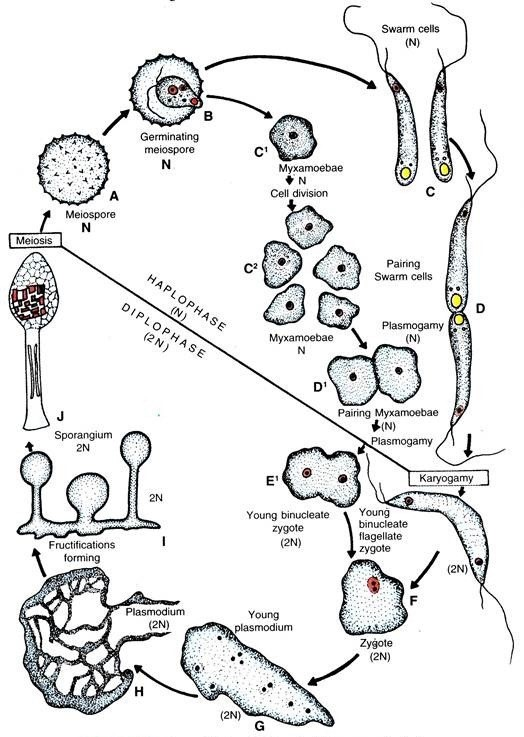
\includegraphics[width = 0.45\textwidth]{images/PhysarumPolycephalum.jpg}
    \caption{The life cycle of \Gls{Physarum polycephalum} \cite{kritartha_life_2016}}
\end{figure}

\Glspl{plasmodial slime mold} are most recognisable during their plasmodial stage, when they exist as a single multinucleated cell. The single cell is filled with a thick soup of molecules and fluid, known as protoplasm \cite{alim_physarum_2013}. \Glspl{plasmodial slime mold} have also been known to grow to impressive sizes, measuring as large as a foot in diameter, impressive since it is a single cell \cite{jabr_how_2012}. When in this stage, \Gls{Physarum polycephalum} uses peristaltic movements of its protoplasm to move \cite{Britannica_slime_2019, alim_physarum_2013}. It will use projections of itself to explore and forage in its surroundings, growing across a space and then reorganising to form a network between food sources \cite{jabr_how_2012, patino-ramirez_substrate_2019}. This is the most impressive behaviour displayed by \Gls{Physarum polycephalum} as it appears to display intelligence, or at the very least a form of problem solving \cite{alim_physarum_2013}.

This is significant since by doing so, \Gls{Physarum polycephalum} very apparently displays emergent behaviour. It allows us an insight into how truly fantastic the phenomenon of emergence is. Intelligence and problem solving are characteristics currently associated with developed frontal and parietal lobes \cite{noauthor_where_nodate}. Despite this, \Gls{Physarum polycephalum} has no nervous system, and with it, a complete lack of any centralised decision-making region including a brain \cite{alim_physarum_2013}.

By forming a network between food sources, \Gls{Physarum polycephalum} is in essence able to solve “the traveling salesman problem”. This mathematical challenge is outlined as follows:

A salesperson has $N$ number of cities to visit and wishes to sell their produce at each location. What is the shortest, and therefore most efficient path for the salesperson to follow?

For a small value of $N$ the challenge is relatively simple to solve. By finding all possible connections of the points, and then choosing the shortest path the problem is quickly solved. However, the complexity of the problem increases exponentially not linearly. Thus, to solve the problem for just a few nodes it could take uncountable iterations. This quickly shows how impressive the task completed by the slime mould is, since the task is in many cases too computationally heavy for a computer using a brute force methodology.

Using this behaviour of \Gls{Physarum polycephalum}, an experiment was devised by Atsushi Tero from Hokkaido University \cite{jabr_how_2012}. Oats were placed on a scale map of Tokyo and its surrounding area, with each oat representing a major station surrounding Tokyo’s city centre \cite{bbc_earth_lab_can_2018}. This changed the implications of the slime molds behaviour; no longer was the slime mold connecting a network of randomly distributed points, but rather it was solving an infrastructure problem that took many engineers, many years to design \cite{bbc_earth_lab_can_2018, world_science_festival_what_2019}; and remarkably, when the slime mold branched out and connected each oat in an intricate network the resulting web almost exactly matched the railway infrastructure \cite{bbc_earth_lab_can_2018, jabr_how_2012}. The slime mold had successfully found the most efficient route between each point.

\section{The Fundamental Algorithm}
\subsection{Ants}
As a starting point, I began by looking at ants, and their use of various chemoattractants to communicate and develop swarm intelligence. Ants have also been shown to solve multiple complex problems including the travelling salesperson problem \cite{httpwwwardamiscom_emergent_2009}, making them an excellent candidate for a first look at algorithmic approximations of emergence. 

My initial algorithm was intended to simulate the movement of a single ant. Each ant would be modelled with a \gls{class}, existing as an individual instance, with their own set of attributes:

\begin{center}
\begin{tabular}{ | m{5em} | m{7cm}| } 
  \hline
  $x,\: y$& acting as relative positions to the origin, in the horizontal and vertical directions respectively, stored as two float/Real numbers \\
  \hline
  $\mathrm{SenseRange}$& which is simply a float number representing how far the ant can detect chemoattractants from \\ 
  \hline
  $v$ & acting as the velocity component for each ant \\ 
  \hline
  $\theta$ & acting as the relative offset in radians with a range of $0 \leq\theta<2\pi$ \\ 
  \hline
\end{tabular}
\end{center}

Every frame, the ant’s relative $x$ and $y$ would be updated in the direction $\theta$ with a magnitude of $v$ (multiplied by the time since the last frame was drawn as to make the simulation frame rate independent), and a marker would be placed to act as a chemoattractant. Once the frame was drawn $\theta$ would be updated to point towards the nearest chemoattractant within a distance of their $\mathrm{SenseRange}$. If no chemoattractant existed, then $\theta$ would remain the same. Finally random variance would be added to $\theta$ allowing variation in the ant’s movement, which would also give rise to a wandering mechanic within the ant’s behaviour, closely modeling the logic behind the implementation of a particle physics simulation \cite{artificial_life_lab_graz_how_2016}.

\subsection{Slime}

I based my overarching logic for my final simulation, upon this principle of independent agents acting together all influenced by their surroundings, but ultimately unaware of the greater simulation.

Very much alike my ant simulation, each agent within the simulation space had two main components that were individual to it:

\begin{center}
\begin{tabular}{ | m{6em} | m{7cm}| } 
  \hline
  $x,\: y$ & acting as two dimensional coordinates relative to the origin, in the horizontal and vertical directions respectively. $\{x,y\} \subset \mathbb{R}$\\
  \hline
  $\theta$ & acting as the relative offset in radians with a range of $0 \leq\theta<2\pi$ \\ 
  \hline
\end{tabular}
\end{center}

On top of this each separately defined species has its own set of attributes that apply to each of the agents assigned to that species of slime mold.

It should be noted that, when I reference species from this point forward, I am not referencing biological species, but rather different permutations of \Gls{Physarum polycephalum} with subtly different settings, leading to different patterns of cohesion and organisation.

\begin{center}
\begin{tabular}{ | m{6em} | m{7cm}| } 
  \hline
  $n$&  denoting the number of agents that will populate the simulation\\
  \hline
  $v$ & the velocity of all agents in the simulation \\ 
  \hline
  $\mathrm{SpawnMode}$ & the initial starting configuration for agents when the simulation starts\\
  \hline
   $\mathrm{DecayRate}$ &  the rate at which chemoattractant fades from the simulation\\ 
  \hline
   $\mathrm{DiffuseRate}$ & the rate at which chemoattractractant spreads across the simulation space \\ 
  \hline
   $\mathrm{SensorOffset}$ & the distance from the agent checked by the algorithm \\ 
  \hline
   $\mathrm{SensorSize}$ & the size of the area of pixels checked by the algorithm\\ 
  \hline 
  $\mathrm{SensorSpacing}$ & the angle between each sensor  \\
  \hline
   $\mathrm{Turn}\: v$ & the speed at which an agent is able to change its relative direction \\ 
  \hline
   $r,\: g,\: b,\: a$ & the red, green, blue and alpha channels used to colour each agent while the simulation is running (useful for distinguishing between different species) \\ 
  \hline
\end{tabular}
\end{center}

\subsection{Textures and Data Storage}
The algorithm is also based on four main render textures: 
\begin{description}
    \item[Trail Texture] stores the agent data and chemoattractant trails.
    \item[Diffused Texture] uses the DiffuseRate to blur the chemoattractant trails before storing the resulting values in each pixel.
    \item[Colour Texture] the diffused texture with a re-colour shader applied, it uses the stored RGBA values within the species data.
    \item[Final Texture] this is the texture rendered to the screen each frame, derived from the Colour Texture.
\end{description}
and the size of the textures is the same between all four. It is the size of these textures that denotes the size of the simulation space. I used 1080 x 920 px as a standard size for all of my simulations. I used each pixel to denote discrete space, leading to a simulation much like John Conway's 'Game of Life'; A cellular automata defined by a set of simple rules \cite{numberphile_inventing_2014, rational_animations_epic_2011}.

When the simulation starts for the first time it calls to the Set method. This method handles the loading of all the data into the simulation, before also passing that same data into each of the \glspl{compute shader} that will handle the simulation and textures.

Once all the relative data is retrieved the algorithm initialises a compute buffer and an array, both set to a size of $n$. The array will store the relative $x$, $y$ and $\theta$ for each agent, while the buffer will do the same for each frame of the simulation, and each texture on that frame.

\subsection{Spawning}

once the data is passed in, and the simulation starts the first frame, the simulation calls to a  function that handles agent setup. The function is passed the array of agents, the width and height of the simulation, and a parameter denoting what spawn mode to start the simulation in. There are four main starting configurations. For each Agent their $x$, $y$ and $\theta$ are set, and the array is returned with updated Agent values.
\begin{description}
    \item[Point] where all agents spawn in a single point at the centre of the simulation space. 
    \begin{equation}
        x=\dfrac{W}{2}
    \end{equation}
    Where $W$ is defined as the width of the simulation space 
    \begin{equation}
        y=\dfrac{H}{2}
    \end{equation}
    Where $H$ is defined as the height of the simulation space
    \begin{gather}
        \theta=2\pi(R)
    \end{gather}
    Where $R$ is some random value unique to each agent, $ 0\leq R \leq 1.0$, $R \in \mathbb{R}$.
    \item[Random] where all agents spawn with a random position within the simulation space
    \begin{equation}
        x = R_{1}
    \end{equation}
    \begin{equation}
        y = R_{2}
    \end{equation}
    \begin{equation}
        \theta = 2\pi(R_{1})
    \end{equation}
    Where $R_{1}$, $R_{2}$ and $R_{3}$ are unique random values, \\
     $0 \leq R_{1} \leq $ Simulation space width, $0 \leq R_{2} \leq$ simulation space height $0 \leq R_{3} \leq 1.0$ \\ 
     $\{R_{1}, R_{2}, R_{3}\} \subset \mathbb{R}$.
    \item[Random Circle] where all agents spawn on a random location within a circle that is $0.15 \times$ the simulation space height, with a random $\theta$.
    \begin{equation}
        x = W + 0.15W(\sqrt{R_{1}}) \cos{(2\pi R_{2})}
    \end{equation}
    \begin{equation}
        y = W + 0.15H(\sqrt{R_{3}}) \sin{(2\pi R_{4})}
    \end{equation}
    \begin{equation}
        \theta = 2\pi(R_{5})
    \end{equation}
    Where $A=\{R_{1},R_{2},R_{3},R_{4},R_{5}\}$,  
    $0 \leq A \leq 1.0$, $A \subset \mathbb{R}$, \\
    $W =$ the simulation space width, and $H =$ the simulation space height
    \item[Inward Circle] where all agents spawn on a random location within a circle that is $0.15 \times$ the simulation space height, and all agents are oriented to face towards the centre of the screen.
     \begin{equation}
        x = W + 0.15W(\sqrt{R_{1}}) \cos{(2\pi R_{2})}
    \end{equation}
    \begin{equation}
        y = W + 0.15H(\sqrt{R_{3}}) \sin{(2\pi R_{4})}
    \end{equation}
    \begin{equation}
        \theta = \arctan\left(\cfrac{
        \cfrac{H\div 2 - y}{\sqrt{(H\div 2 - y)^{2} + (W\div 2 - x)^2}}}{
        \cfrac{W\div 2 - x}{\sqrt{(H\div 2 - y)^{2} + (W\div 2 - x)^2}}}
        \right)
    \end{equation}
    Where $A=\{R_{1},R_{2},R_{3},R_{4},R_{5}\}$,  
    $0 \leq A \leq 1.0$, $A \subset \mathbb{R}$, \\
    $W =$ the simulation space width, and $H =$ the simulation space height
\end{description}

Following the assignment of the Agent data, the array data is passed into the agent compute buffer. Where the main simulation \gls{kernel} is given the starting values of all the Agents. On the first frame the starting configuration acts as the data that is rendered to the screen without the simulation running. This involves simply passing the Agent data into into the main kernel where the texture is directly copied onto the final texture, and each pixel is coloured white for each agent's respective $x$ and $y$, while the rest of the texture remains black.

\subsection{Running the Simulation}

for all following frames the data is passed to the Run Simulation Method:

This method handles all data for the simulation, and manages the movement of data between kernels and the main program. foremost it checks that the Trail Texture does not equal null. Should it be found that the Trail Texture does not exist, the trail texture is initialised to a new RenderTexture object. The Render texture is set to use \Gls{RGBA} colour space, and random read and write is enabled. Finally the filter mode is set to \gls{bilinear}, and the texture is created.

This same process is repeated for each texture.

Following the creation of these textures, all the textures are assigned to their corresponding kernels. and each of the compute shaders are dispatched. Including:
\begin{description}
    \item[pragma kernel Update] Which handles the behaviour for each Agent, based on their $\theta$ and local \gls{chemoattractant} intensity.
    \item[pragma kernel Diffuse] Blurs the entire texture with an averaging algorithm.
    \item[pragma kernel ReColour] takes the relative value from 0 to 1 for each pixel and finds the dot product with $r, g, b,$ and $a$ to obtain a re-coloured version of the diffused texture.
\end{description}

Finally the method finishes by copying the diffused texture to the trail texture, and the Colour texture to the final texture. This is accomplished with a function that simply transfers data from the source texture to the target texture. 

\subsection{Pragma Kernels}
\subsubsection{Update}

The Update kernel foremost checks that the current id $\not\geq n$.

Following this it generates a pseudo random value from a predetermined hash function, the hash function receives a single seed:
\begin{equation}
    RandomValue = \frac{ffg(seed)}{4294967295}
\end{equation}

where $RandomValue$ has a range of $R:[0,1]$, and the functions $g$ and $f$ are defined as: 
\begin{equation}
    g(x) = 2654435769\left(x ^{2747636419}\right)
\end{equation}
\begin{equation}
    f(x) = 2654435769\left(x^{(x \gg 16)}\right)
\end{equation}

To calculate a value for each individual agent the hash function is iterated on twice, using the first hashed value to generate a seed for the final random value that will be used by that agent for that frame of the simulation.

\begin{equation}
    RandomValue = \frac{ffg\left(y \times width + x + \frac{ffg(x + (time \times 100000))}{4294967295}\right)}{4294967295}
\end{equation}

The next key part of the algorithm for agent behaviour is the sense function. This function acts as the main vision for the Agent. The method is passed both the Agent in reference, and a sensor angle offset.

\begin{center}
\begin{tabular}{ | m{8em} | m{7cm}| } 
  \hline
   Sensor Angle & defined as $\theta$ + sensor angle offset. This will act as the relative offset based on the Agent's relative facing. \\
  \hline
   $SensorCenterX$ &  defined as $\cos{(Sensor Angle)}$\\ 
  \hline
   $SensorCenterY$ &  defined as $\sin{(Sensor Angle)}$\\ 
  \hline
   sum & used as a running total for the overall weight of that relative area.\\ 
  \hline
\end{tabular}
\end{center}

The sense method checks a square of size SensorSize, centered on $(SensorCenterX, SensorCenterY)$. The algorithm loops through each pixel individually, within the allocated size. In order to account for index values that could be greater than the size of the simulation space the $x$ and $y$ coordinates for each pixel to be used are first checked, and corrected. The $x$ and $y$ coordinates are defined as:

\begin{equation}\label{xbound}
    x = \min(width -1, \max(0, x))
\end{equation}
\begin{equation}\label{ybound}
    y = \min(height - 1, \max(0, y))
\end{equation}

Following the calculation of the $x$ and $y$ coordinates for each pixel, the sum is incremented by the value of the chemoattractant stored in the pixel with the respective coordinates. It is this sum value that is returned by the sense method. Due to this edge detection algorithm the chemoattractant in each of the boarder pixles does have the potential to have as much as the weighting multiplied by the SensorSize$^2$, dependent on the location of the sensor. 

Back within the main Update kernel, following the generation of the pseudo random number, the main rules for movement are outlined. Foremost three areas are sampled; using the sense method, the kernel stores three values to represent each 'chunk' of vision available to the Agent. The first area is directly ahead of the Agent, where the sense method is passes a sense angle offset of zero. Following this each of the remaining two sections are passed $\pm$ SensorSpacing to rotate the region of focus both clockwise and anti-clockwise. This  results in the centers of each region having a radial distance of SensorSpacing between each of them.

The next phase of the kernel handles which direction the agent will face based on the results from the Sense regions. In the case that there is the strongest quantity of chemoattractant directly ahead, $\theta$ is not changed. In the case that either the clockwise, or anti-clockwise regions is more heavily weighted than the other, then $\theta$ will be updated. $\theta = \theta \pm (RandomValue \times TurnSpeed)$. It is the random value that adds enough variation as to allow the simulation to evolve organically over time. In the occasion that both the clockwise and anti-clockwise regions have equal values then a random turn value is calculated to prioritise a single direction over another for that frame, this constitutes the random searching behaviour of each agent.

\begin{equation}
    \theta = \theta + \left(2(TurnSpeed) \times (RandomValue - 0.5)\right)
\end{equation}
    
Following this the new $x$ and $y$ are calculated based on the facing direction of the agent.The next pixel the Agent occupies is then calculated as:

\begin{equation}
    x = x + \left(\cos{(x)}\times v \times \delta\right)
\end{equation}
\begin{equation}
    y = y + \left(\sin{(x)}\times v\times\delta\right)
\end{equation}

Where $\delta$ is defined as the time since the last frame. This multiplication scales the movement by the relative frame rate. Allowing the movement of the Agent to be independent of the frame rate.

The next crucial step is to confine the agents to the simulation space. If the target pixel is located outside the bounds of the texture then a new position is calculated. First the random value is recalculated.

\begin{equation}
    RandomValue = \frac{ffg\left(RandomValue \times 4294967295 \right)}{4294967295} \times 2 \pi
\end{equation}

This prevents the same random value from being used a second time over and scales it to a range of $R: [0,2\pi]$.

I used much of the same logic as for if the pixel was outside of the search range within the sense function, whereby the $x$ and $y$ are reset to pixels within the simulation space using the same algorithms \eqref{xbound}\eqref{ybound}, and $\theta$ is reset to face a random direction. This can result in the Agent leaving the simulation space again. However, probability dictates that eventually the agent's $\theta$ will be reset to a value that allows it to re-enter the simulation. 

\begin{equation}
    \theta = RandomValue
\end{equation}

This set of equations will only run if the Agent is found to occupy a pixel outside the simulation, saving the kernel from excess computation.

The final and most important step taken by this kernel is to update the Trail Texture. This is done by finding the Trail Texture pixel with location $x$ and $y$. The value of this cell is set to 1 in all RGBA channels, this essentially colours the associated pixel white. This step is significant as it acts as the primary record of the location of each agent, including where they have been over time. Since this Texture is updated each frame, the path of each agent can be followed by tracing the path of white pixels.

\subsubsection{Diffuse}

The next step for the simulation is to pass the data from the Trail Texture into the Diffuse kernel. This kernel uses two main real numbers, a value for the DiffuseRate and a value for the DecayRate. A significant feature of this kernel, is its dependence on the Trail Texture. However, as a rule, the Diffuse kernel is unable to write to the Trail Texture, rather it creates its own texture map that inherits all the data from the Trail Texture. This avoids conflicts of data on the GPU allowing for more sequential assignment of data between frames, it is this texture that is defined as the Diffused Texture.

To apply the necessary blur to the texture the following algorithm is applied:

\begin{center}
\begin{tabular}{ | m{8em} | m{7cm}| } 
  \hline
   Original Weight & defined as the weight of the cell from the Trail Texture that is currently being iterated over. \\
  \hline
   Blurred Colour &  defined as the sum divided by the scale of the blur.\\ 
  \hline
   Diffuse Weight &  used as the weight of diffusion for that frame in reference real time.\\ 
  \hline
   sum & used as a running total for the overall weight of that relative pixel.\\ 
  \hline
\end{tabular}
\end{center}

We start by initialising the value of sum to 0, and Original Weight to the value of our pixel from the Trail Texture. Following this, we iterate over a three by three pixel grid centred on our target pixel. We clamp our pixels to sit within the simulation space using the same algorithm as in our sense function \eqref{xbound}\eqref{ybound}. Following this we set our sum to the sum of each cell within the three by three grid, assuming each pixel is not outside the bounds of the simulation space. This algorithm does again more heavily weight pixels on the edge of the simulation. Blurred Colour is then set to store the average of each of these cells accomplished as,
\begin{equation}
    BlurredColour_1 =\cfrac{sum}{9}
\end{equation}

Diffuse Weight is then calculated as
\begin{equation}
    DiffuseWeight = \min{(1, \max{(0, DiffuseRate \times \delta)})}
\end{equation}

Where $\delta$ is the time since the last frame was drawn, this addition keeps the diffusion of chemoattractants independent of frame rate, again allowing for real time rendering.

Finally Blurred Colour is recalculated as
\begin{equation}
    BlurredColour_2 = OriginalColour \times (1 - DiffuseWeight) + BlurredColour_1 \times DiffuseWeight
\end{equation}

The pixel in Diffused Texture is then set to:
\begin{equation}
    \max{(0, BlurredColour_2 - DecayRate \times \delta)}
\end{equation}

Where $\delta$ is the time since the last frame was drawn. This final calculation is used to fade the \gls{chemoattractant} from the scene while also clamping the value to a range of $D:[0,1]$.

The most crucial step outside of the kernels to take place between each frame is the copying of the Diffuse Texture to The Trail Texture, this is the fundamental step that defines how the Agents react to and set down \glspl{chemoattractant}.

\subsubsection{Recolour}

The final kernel to address is the ReColour kernel. This phase is entirely optional, as it simply applies a colour to the simulation, this helps to determine between different species of slime mold, but is essentially aesthetic. The kernel takes an input of each pixel and divides each colour channel into their respective value. Since the simulation runs off of single values all the corresponding channels will be identical to begin with, this lack of complexity makes re-colouring very simple. I simply calculate each channel as
\begin{equation}    
    Channel = value \cdot colour
\end{equation}

Where $Channel$ represents each of the RGBA channels. $value$ represents the numerical value stored in each cell of the simulation, and $colour$ is the target colour when  $value = 1$.

To finish the entire single iteration of a frame, the re-coloured texture is copied to the Final Texture which is rendered to the screen.

\section{Implementation}

I found with my implementation, the sensitivity of the simulation very closely resembled the characteristics of a chaotic system; the tiniest change in settings, results in vastly different outcomes. The largest impact I found was associated with the cohesion of the Agents. This was impacted by a culmination of each of the settings acting in unison, as seen in figure  \ref{fig:EPQ} particularly between examples such as figure \ref{fig:EPQ_4} and figure \ref{fig:EPQ_6}.

\begin{figure}
    \centering
    \begin{subfigure}{0.3\textwidth}
        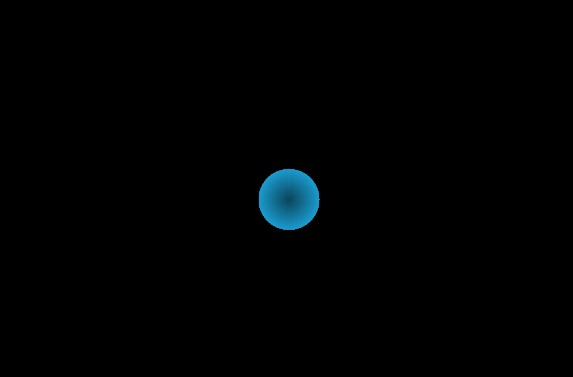
\includegraphics[width=0.9\linewidth]{images/EPQ 1.jpg}
        \caption{The starting frames of a slime mold with high cohesion and a spawn mode of point}
        \label{fig:EPQ_1}
    \end{subfigure}
    \hfill
    \begin{subfigure}{0.3\textwidth}
        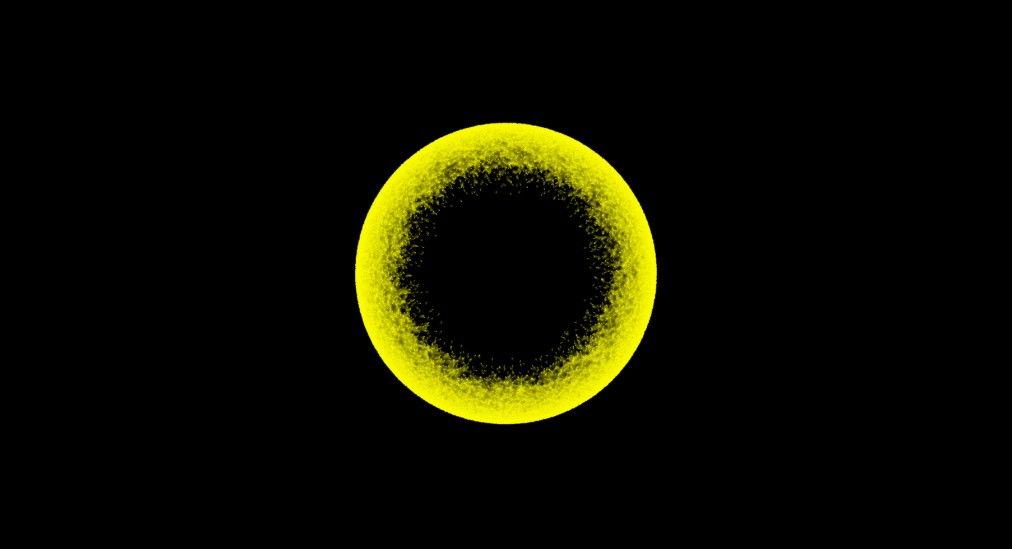
\includegraphics[width=0.9\linewidth]{images/EPQ 2.jpg}
        \caption{a slime mold with high cohesion but low sense range and turn speed}
        \label{fig:EPQ_2}
    \end{subfigure}
    \hfill
    \begin{subfigure}{0.3\textwidth}
        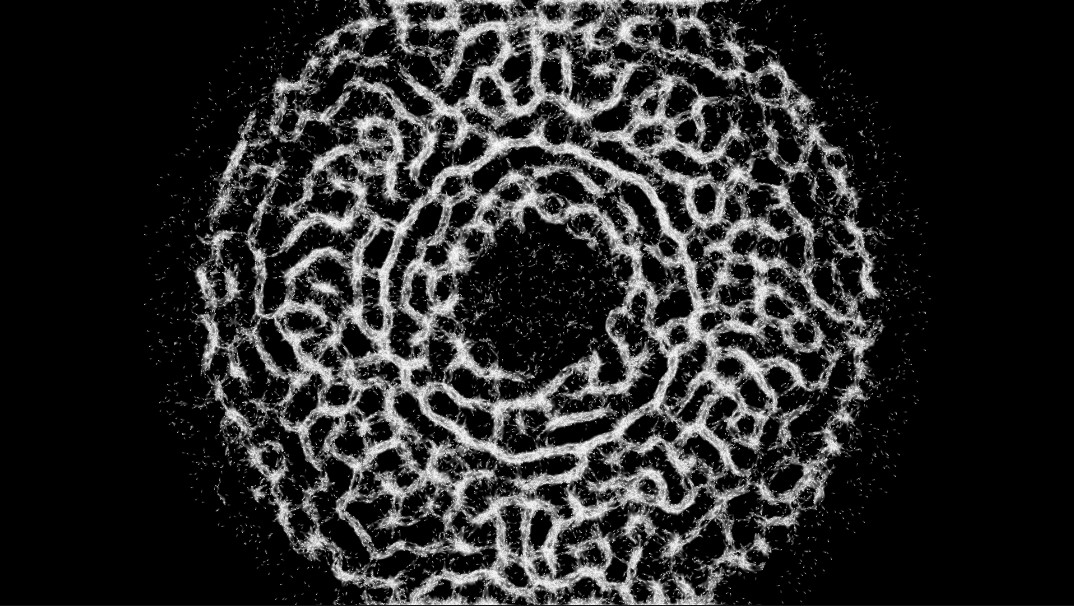
\includegraphics[width=0.9\linewidth]{images/EPQ 3.jpg}
        \caption{this species has a very high cohesion but a quite limited sense range while also moving very slowly.}
        \label{fig:EPQ_3}
    \end{subfigure}
    \hfill
    \centering
    \begin{subfigure}{0.3\textwidth}
        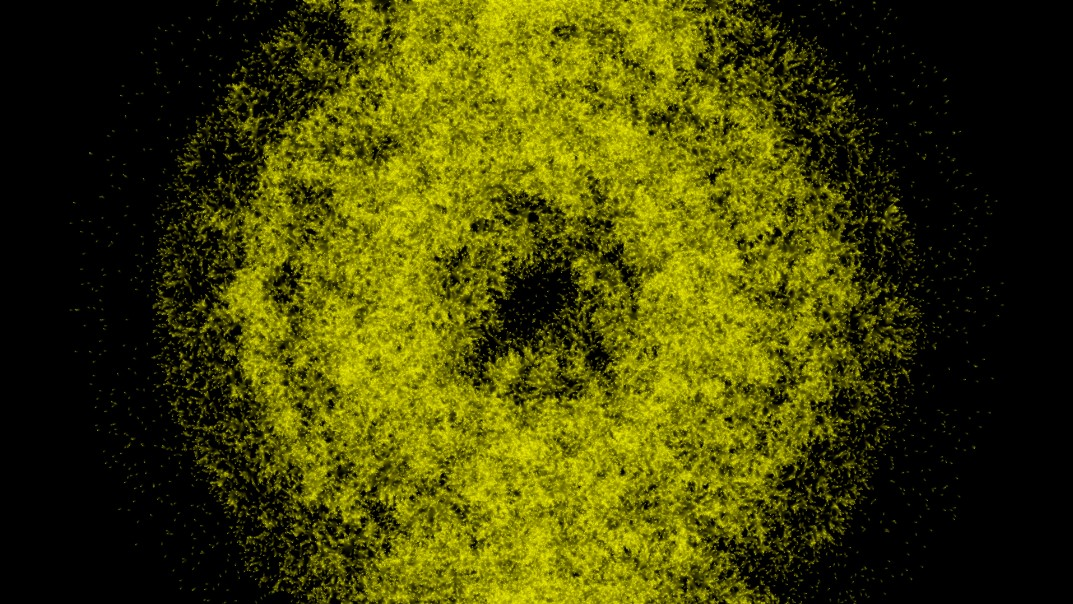
\includegraphics[width=0.9\linewidth]{images/EPQ 4.jpg}
        \caption{this species has almost no vision, leading to a complete lack of cohesion}
        \label{fig:EPQ_4}
    \end{subfigure}
    \hfill
    \begin{subfigure}{0.3\textwidth}
        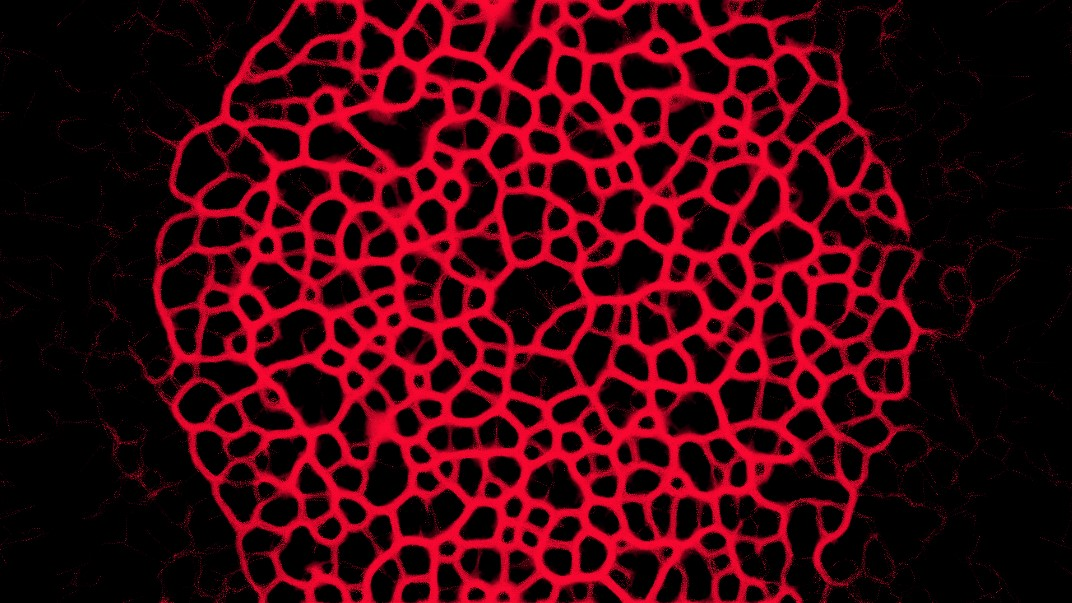
\includegraphics[width=0.9\linewidth]{images/EPQ 5.jpg}
        \caption{this species exhibits the closest and most accurate portrayal of behaviours exhibited by \Gls{Physarum polycephalum}}
        \label{fig:EPQ_5}
    \end{subfigure}
    \hfill
    \begin{subfigure}{0.3\textwidth}
        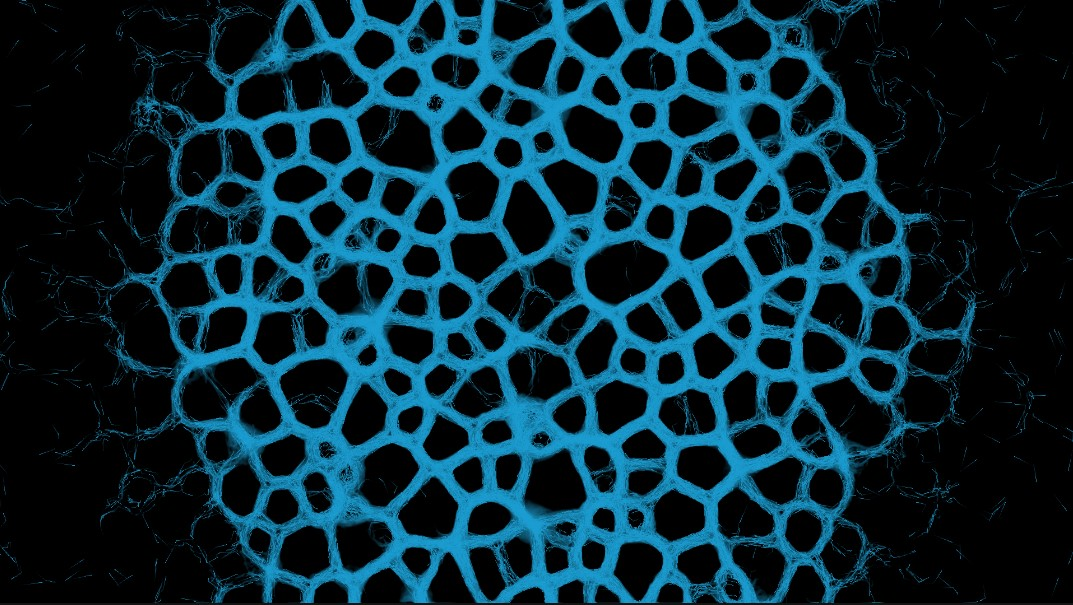
\includegraphics[width=0.9\linewidth]{images/EPQ 6.jpg}
        \caption{this species has fantastic sense range and size, and can move comparatively very quickly leading to harsher shapes}
        \label{fig:EPQ_6}
    \end{subfigure}
    \caption{A series of frames from my simulation exhibiting different species with different behaviours as a result. (Each frame was taken at a different stage in each of the simulations to best showcase the behaviours)}
    \label{fig:EPQ}
\end{figure}

One of the largest changes with my implementation to the final algorithm was, without a doubt, my addition of colour fading. (When switching between different species). This was implemented to account for live displays of my simulation, allowing me to change the settings of the simulation while it was still running. 
This change was purely aesthetic and did not change the behaviour of the simulation at all, but I felt it was important, since I denoted different species with different colours, and I felt a fade between colours was the most visual way to denote a change of settings within the simulation.

\section{Evaluation}
Overall, I am really happy with the result of my simulation. In a lot of different configurations the core behaviors of my simulation matched the interactions of \Gls{Physarum polycephalum}, and most of the patterning formed by the simulation match its organic counterpart. While it only inhabits a 2D plain, the simulation displays organisation, and cohesion, leading to complex pattern formation in the form of a network that continuously changes in response to external stimuli. I feel that in this way I have managed to simulate a close approximation to \Gls{Physarum polycephalum} and the emergence it displays.

Emergence, is a fundamental and complex part of our universe, it is present in all things, and working towards understanding this phenomenon, not only gives us insight into the complexities of organisms such as \Gls{Physarum polycephalum}, but a greater understanding of the complexities of the wider world that surrounds us.

\nocite{*}

\printbibliography
\addcontentsline{toc}{chapter}{Bibliography}

\end{document}
